%  !TeX  root  =  user_guide.tex

\section{Spatial Query Plugin}\label{sec:spatial_query}

% when the revision of a section has been finalized, 
% comment out the following line:
% \updatedisclaimer

The \toolbtntwo{spatialquery}{Spatial Query} plugin allows to make a spatial 
query (select features) in a target layer with reference to another layer. The 
functionality is based on the GEOS library and depends on the selected source 
feature layer. 

Possible operator are:

\begin{itemize}[label=--]
\item Crosses
\item Intersects
\item Is disjoint
\item Touches
\item Within
\end{itemize}

Polygon layers do not provide the 'Touches' and 'Crosses operator.

\minisec{How to use the plugin}

As an example we want to find regions in the Alaska dataset that contain 
airports. Following steps are necessary:

\begin{enumerate}
  \item Start QGIS and load the vector layers regions.shp and airports.shp. 
  \item Load the Spatial Query plugin in the Plugin Manager (see Section 
  \ref{sec:load_core_plugin}) and click on the \toolbtntwo{spatialquery}{Spatial Query}    
  icon which appears in the QGIS toolbar menu. The plugin dialog appears as shown 
  in Figure \ref{fig:spatialquerysample}.
  \item Select layer regions as source layer and airports as reference feature layer.
  \item Select 'Contains' as operator and click \button{Apply}.
\end{enumerate}

Now you get a list of feature IDs from the query and you have several options.

\begin{itemize}[label=--]
\item Click on the \toolbtntwo{selectesubsetlayer}{Create layer with list of items}
\item Select an ID from the list and click on \toolbtntwo{selectcreatelayer}{Create layer with selected}
\item Select the \button{Remove from current selection} in the field 'And use the 
result to'.
\item Additionally you can \checkbox{Zoom to item} or display \checkbox{Log messages}.
\end{itemize}

\begin{figure}[ht]
   \centering
   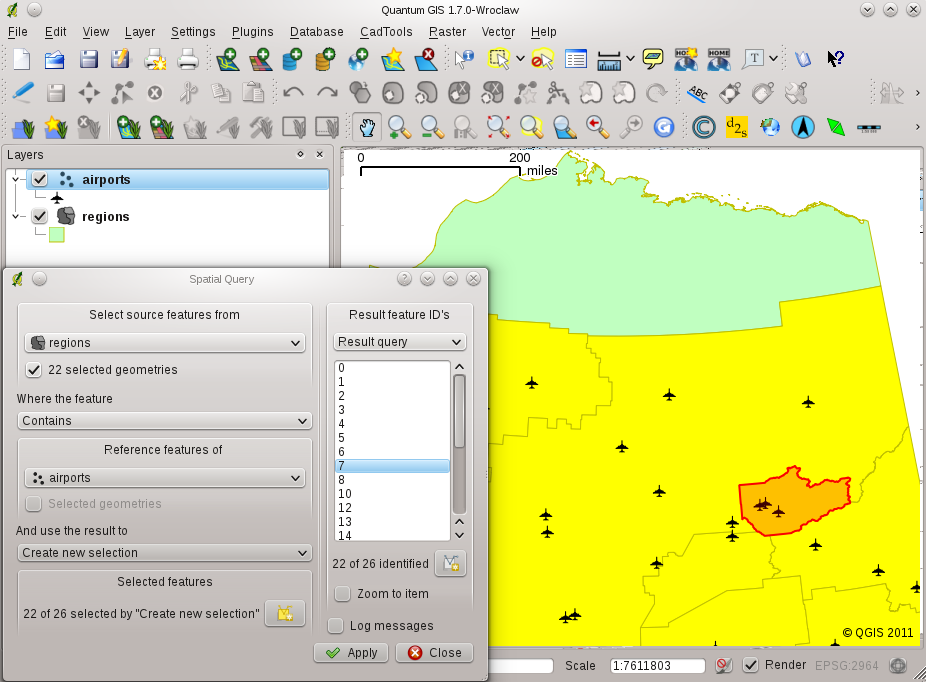
\includegraphics[clip=true, width=14cm]{spatial_query_sample}
   \caption{Spatial Query analysis - regions contain airports \nixcaption}
   \label{fig:spatialquerysample}
\end{figure}

\FloatBarrier

